
%(BEGIN_QUESTION)
% Copyright 2006, Tony R. Kuphaldt, released under the Creative Commons Attribution License (v 1.0)
% This means you may do almost anything with this work of mine, so long as you give me proper credit

Shown here is the response of a proportional+derivative controller to a ramping process variable (with a constant setpoint).  Calculate the controller's proportional and derivative constant settings, based on what you see in the graph.  Also, determine whether this controller is direct or reverse acting, and mark the features of the output plot corresponding to proportional action and to derivative action.

$$\includegraphics[width=15.5cm]{i01544x01.eps}$$

The time scale on the chart is minutes:seconds, and the P+D algorithm is as follows:

$$m = K_p \left( e + \tau_d {de \over dt} \right) + b$$

\noindent
Where,

$m$ = Controller output (manipulated variable)

$K_p$ = Gain

$e$ = Error signal (SP$-$PV or PV$-$SP)

$\tau_d$ = Derivative time constant

$b$ = Bias

\vskip 10pt

Also, determine the gain and derivative constant values if you were told the PD algorithm were this instead:

$$m = K_p e + \tau_d {de \over dt} + b$$

\underbar{file i01544}
%(END_QUESTION)





%(BEGIN_ANSWER)

Controller action = {\it direct}

\vskip 10pt

$K_p$ = 0.5 (proportional band = 200\%)

\vskip 10pt

$\tau_d$ = 1 minute = 60 seconds

\vskip 10pt

$$\includegraphics[width=15.5cm]{i01544x02.eps}$$

If the other algorithm were used, the gain and derivative constants would be:

\vskip 10pt

$K_p$ = 0.5 (proportional band = 200\%)

\vskip 10pt

$\tau_d$ = 0.5 minute = 30 seconds

%(END_ANSWER)





%(BEGIN_NOTES)


%INDEX% Control, proportional + derivative: graphing controller response

%(END_NOTES)


